\section{The microscopic description of atomic systems}
Molecular dynamics, and computational statistical physics at large, aim at simulating on the computer the behavior of physical systems.
The hope is that one can infer quantities and properties of real-life interest from observing the results of numerical simulations, which may be relevant to understand the material properties of many-particle systems, or the nature of interactions in complex systems such as those found in biology.
Computational simulations can thus act as surrogate experiments in cases where experimental setups are hard to achieve, or measurements are impossible.
They can also be seen as surrogate tests of theoretical models, as they allow to test the validity of a mathematical description by comparing numerical predictions to experimental data. Molecular dynamics, in particular, is concerned with simulating atomic systems, most often (and as we shall systematically do) using a classical description.

\subsection{Classical phase space}

We consider a system of $N$ particles evolving in $d$-dimensional space.
The classical description contends that the \textit{state} of a system is the datum of the positions and momenta of every particle in the system.
We can interpret this as the statement that, given full knowledge of the positions and momenta at some initial time, and of the forces at play, one can deduce exactly the positions and momenta at any future time.
It is often the case in computer simulations that we consider positions which are restricted to a bounded domain by the use of periodic boundary conditions. To that effect, let
$$ \mathcal D = (L\mathbb T)^{dN} \text{or } \R^{dN}, $$
where $\mathbb T$ is the one-dimensional torus. We call $\mathcal D$ the configuration space.

\begin{definition}[Phase space]

    We describe the positions and momenta of the atoms as vectors
    $$ q=(q_{1,1},\dots,q_{1,d},\dots ,q_{N,1},\dots,q_{N,d})^\intercal \in \mathcal D,$$
    $$ p=(p_{1,1},\dots,p_{1,d},\dots ,p_{N,1},\dots,p_{N,d})^\intercal \in \R^{dN},$$

    where $q_i \defeq (q_{i,1},\dots, q_{i,d})^\intercal$ is the position vector of the $i$-th particle, and similarly for $p$. Let

    $$\mathcal E \defeq \mathcal D \times \R^{dN}.$$
\end{definition}

Central objects in our study will be trajectories 
$$(q_t,p_t)_{t\geq 0} \subset \mathcal E,$$
which describe the time evolution of a physical system.

It is not clear \textit{a priori} why we should choose momenta to describe the kinetic quality of the system, rather than velocities. However it is of no importance since we can change from one description to the other via the relation
$$v=M^{-1}p,$$
where $M\in \R^{dN \times dN}$ is a diagonal matrix recording the masses of each particle ($d$ times per particle), and $v$ is the velocity vector.

\subsection{Dynamical description}

In order to describe the evolution of the system's state, one must specify a dynamical law. This is done by giving a function
$V: \mathcal E \to \R$ whose gradient in the $i$-th particle's coordinates 
$$ \nabla_{q_i} V \defeq (\partial_{q_{i,d}},\dots , \partial_{q_{i,d}})^\intercal $$
gives minus the force vector acting on the $i$-th particle. In our case we will always take the potential to be independent of the momentum, so that we can think of $V$ as having domain $\mathcal D$. In the case where $\cD = (L\mathbb T)^{dN}$, it will be convenient to think of $V$ as a function from $\R^{dN}$ to $\R$ which is $C^1$ and $L$-periodic in each direction.
The function $V$ is called the potential, and, as it encodes the dynamics of the system, it is of paramount importance. The time evolution of the system, then, is described by Newton's second law:

$$\frac{\text{d} p}{\dt}=-\nabla V(q)$$.

It will be convenient for our analysis to use of reformulation of Newton's equations, based on the Hamiltonian of a system.

\begin{definition}[Hamiltonian]
    The Hamiltonian of a classical system is its total energy, which is the sum of a kinetic energy term depending only on the momenta and a potential energy term depending only on the positions.

    \begin{equation}
        \label{eq:hamiltonian}
        H(q,p)=\frac12p^\intercal M^{-1}p+V(q)
    \end{equation}
\end{definition}

Using the Hamiltonian, we can rewrite the classical equations of motion as

\begin{equation}
\label{eq:hamiltonian_dynamics}
\begin{cases}
    \mathrm{d} q_t=M^{-1}p_t\dt=\nabla_p H(q_t,p_t)\dt\\
    \mathrm{d} p_t=-\nabla V(q_t)\dt=-\nabla_q H(q_t,p_t)\dt
\end{cases},
\end{equation}

The potential is the most important part of the microscopic description, and accordingly, the main problem in establishing a physical model of this kind is to determine potential functions which adequately capture the dynamic behavior of a given system. 
The choice of a classical description automatically implies a degree of approximation, since behavior arising from the laws of quantum mechanics, which may be relevant at a microscopic level, are described by Newton's law.
 Furthermore, if the aim is to simulate such systems numerically, computational constraints imply that some compromise has to be reached between theoretical accuracy and computational cost. 
 If, for small systems, it may be possible to simulate all atomic interactions, for larger or more complex systems, it is often to use potential functions which are both cheap from a computational point of view and empirically shown to be accurate enough for the purpose of a simulation.
 
 Our main numerical example will be the system given by the following potential, which is of this empirical form, and which is often used to describe the microscopic behavior of chemically inert fluids, such as Argon.

 \begin{example}[The Lennard-Jones fluid]
    We fix $L>0$, $d=3$, and $N$ the number of particles. The Lennard-Jones fluid is the classical system given by the pair-interaction potential

    \begin{equation}
        \label{eq:lennard_jones}
        V_{\mathrm{LJ}}(q)=\sum_{1\leq i < j \leq N} v(|q_i-q_j|),        
    \end{equation}

    where $v$ is a radial function

    $$v(r)=4\varepsilon \left( \left( \frac{\sigma}{r}\right)^{12}-\left(\frac{\sigma}{r} \right)^6\right).$$

    The reference energy $\varepsilon$ and length $\sigma$ are shape parameters which respectively control the depth of the potential well of $v$ and the equilibrium distance $2^{1/6}\sigma$.
    As seen on Figure \ref{fig:lennard_jones}, the potential combines two effects. At small interparticular distances, the dominant term is in $r^{-12}$, which translates into a strongly repulsive force between close pairs of particles, and makes individual particles essentially impenetrable.
    At long range, the dominant term is in $-r^6$, which translates into a weakly attractive force between distant particles. Contrary to the repulsive term, which is empirical, this scaling has a theoretical origin in the Van der Waals forces.
    From a computational standpoint, the fact that $v$ is an even function of $r$ allows one to compute the normalized force while sparing the expense of computing a square root, while the identity $r^{12}=(r^6)^2$ allows further economy.
    The shape parameters $\sigma$ and $\varepsilon$ must be chosen empirically to describe the behavior of a particular atomic species. For Argon, values of reference are: $\sigma=$ , $\varepsilon=$.
 \end{example}

 \begin{figure}[htbp]
    \begin{center}
      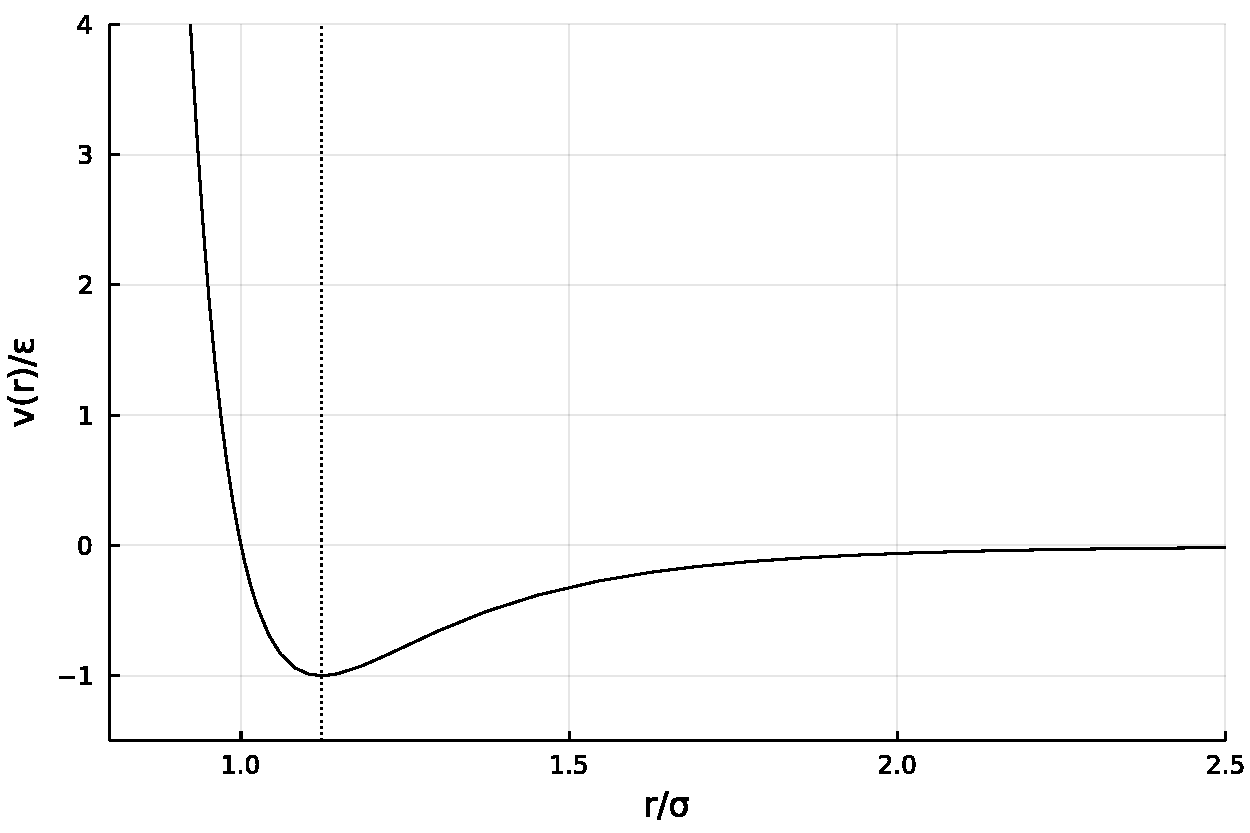
\includegraphics[width=0.7\linewidth]{figures/chapter1/lennard_jones.pdf}
      \caption{ \label{fig:lennard_jones}
        The pair potential $v$, with lengths and energy given in reduced units. The equilibrium interparticular distance is indicated by the vertical dotted line.
      }
    \end{center}
  \end{figure}

\subsection{Reduced units}
It is convenient, given an atomic system, to describe quantities therein within a system of units in which they are of order one. This has several advantages. 
Firstly, like any reasonable system of units, they make quantities easier and more intuitive to reason about.
Secondly, from the computational point of view, numerical artifacts due to loss of precision at very large or very small scales and overflow errors can be avoided more often.
Thirdly, they may help transfer knowledge about one system to another. 
For instance, in the Lennard-Jones system, expressing a quantity in reduced units,
and knowing the dependency of these units on the parameters $(\varepsilon,\sigma,M)$ of the system, one can infer properties about a system with parameters $(\tilde\varepsilon,\tilde\sigma,\tilde M)$ by applying the inverse transformation, thus effectively yielding equivalence of different systems under different conditions, and sparing the cost of running redundant simulations.

We describe a general procedure to construct a set of reduced units. Our choice, although not necessarily unique, is quite natural, especially when dealing with the Lennard-Jones system.
Let us fix a reference mass $m_*$, a reference energy $\varepsilon_*$ and a reference length $\sigma _*$. Then various reference quantities can be derived by natural conversions and dimensional analysis:
\begin{align*}&t_*=\sqrt{\sigma_*^2m_*\varepsilon_*^{-1}},\tag{time}\\
    &T_*=\varepsilon_*k_B^{-1},\tag{temperature}\\
    &v_*=\sigma_*t_*^{-1},\tag{velocity}\\
    &V_*=\sigma_*^3,\tag{volume}\\
    &A_*=\sigma_*^2,\tag{area}\\
    &\rho_*=V*^{-1},\tag{density}\\
    &F_*=m_*\sigma_*t_*^{-2},\tag{force}\\
    &P_*=F_*A_*^{-1},\tag{pressure}
\end{align*}
and one can of course go on. The point is that if $X$ is a quantity, one can obtain its reduced value $X_{\mathrm{red}}$ by dividing $X$ by the reference quantity $X_*$ which is dimensionally compatible with $X$, and which can be derived as above.
For instance, given a pressure $P$, we obtain
$$P_{\mathrm{red}}= P\sigma_*^3\varepsilon_*^{-1}.$$
Note this is an adimensional quantity. Note, also that, due to the definition of the reference temperature $T_*$ relative to the reference energy $\varepsilon_*$, energy are now commensurate to temperatures.
The Boltzmann factor, which is the conversion factor between units of temperature and units of energy simplifies when expressed in reduced units, a fact we can capture with the maxim ${k_B}*=1$. This simplifies many formulae.

For a monoatomic Lennard-Jones system, a natural choice for $m_*$ is the atomic mass of the considered species. We also take $\varepsilon_*=\varepsilon$ and $\sigma_*=\sigma$, (although the equilibrium length $\sigma=2^{1/6}\sigma$ is another possible choice). In the case of Argon, we use the following values:
$$m_*=6.634 \times 10 ^{-26} \text{kg},\ \sigma_*=3.405 \times 10^{-10} \text{m},\ \varepsilon_*=1.66 \times 10^{-21} \text{J}.$$
Unless explicitly specified, all numerical results will be in this system of reduced units.

\section{Statistical ensembles}
The microscopic description is interesting from a theoretical standpoint, but it fails to be relevant when attempting to describe the behavior of atomic systems with a macroscopic number of particles, of the order of Avogadro's number ($6.02 \times 10^{23} $).
Besides the technical impossibility of measuring to a high accuracy the configuration of such systems, and that of recording the information required to track it (coincidentally, the total amount of digitally stored information on Earth is estimated to be $10^{23}$ bytes as of 2022), it is also the case that knowledge of a system at this level of detail is unnecessary to describe the quantities which are relevant to our macroscopic experience.
In the instance of a gas at thermal equilibrium, examples of relevant quantities are total energy, pressure, temperature, density, which, while of course resulting from the internal state of the system, are independent of the minutiae of individual atomic motions: loosely speaking, one may describe the macroscopic state of a system by only a handful of macroscopic variables, loosing track of the myriad of microscopic degrees of freedom.
An important point is that for a given macroscopic state, there are many microscopic configurations which are compatible with our observations. This motivates defining the macroscopic state of a system as a probability distribution over phase space, which we may interpret as assigning to each microscopic configuration a likelihood that this configuration underlies the macroscopic state.

This does not tell one how to choose the distribution over microscopic states. However, it seems reasonable to assign positive probabilities to states compatible with the macroscopic constraints, and in such a way as to make the weakest possible assumptions on this microscopic state, or in other words contain the least amount of information about the system, given the macroscopic constraints. The mathematical translation of this idea is given by the principle of maximal entropy. Given a class of probability distributions compatible with the macroscopic constraints, define the macroscopic state as the one which maximizes the entropy, which is defined for a probability distribution $\rho$ by

\begin{equation}
    \label{eq:entropy}
    \mathfrak S(\rho)=-\int_{\mathcal E} \rho(x)\ln(\rho(x))\dx.
\end{equation}

The specification of a probability distribution over states is called a thermodynamic ensemble. We will be considering the following two examples.

\subsection{Microcanonical ensemble}

    The microcanonical ensemble is the suitable model for an isolated system in thermodynamic equilibrium, evolving under Hamiltonian dynamics. The number of particles $N$, the volume $V=L^3$, and the energy $E$ is fixed. We will alternatively refer to the microcanonical ensemble as the NVE ensemble.
     Because the constant energy condition constrains the compatible microstates to level sets of $H$, which in general will be negligible subsets of $\mathcal E$, some care must be taken in defining the microcanonical measure, since one cannot express the macroscopic constraints by a family of probability densities.
      However, under suitable assumptions on $V$, one can define the microcanonical measure as a weak limit of uniform distributions over level \textquote{shells} of $H$:
    $$\int_\mathcal{E} \varphi\, \mathrm{d}\mu_{\mathrm{mc,E}} \defeq \underset{\varepsilon \to 0}{\mathrm{lim}}\, \frac{1}{|S(E,\varepsilon)|}\int_{S(E,\varepsilon)} \varphi(q,p) \mathrm{d} q \mathrm{d} p,$$
    where 
    $$S(E,\varepsilon) = \{ (q,p) \in \mathcal E |\ H(q,p) \in [E-\varepsilon,E+\varepsilon]\}.$$
    
    This is consistent with the fact that, for a set $A$ with finite Lebesgue measure, the probability distribution on $A$ which maximizes the entropy is the uniform distribution on $A$. 
    Alternatively, $\mu_{\mathrm{mc,E}}$ is uniquely defined by the relation
    \[\int_{\mathcal E}g(H(q,p))f(q,p)\,\mathrm{d}q\mathrm{d}p=\int_{\R}g(E)\int_{\mathcal E} f(q,p)\,\mu_{\mathrm{mc,E}}(\mathrm{d} q,\mathrm{d}p),\]
    for all test functions $g:\,\R\to \R$ and $f:\,\mathcal E\to \R$.
    It is possible, using the coarea formula, to derive an explicit formula for $\mu_{\mathrm{mc,E}}$, namely,

    \begin{equation}
        \label{eq:microcanonical_measure}
        \mu_{\mathrm{mc,E}}(\dif q,\dif p)=\frac{\sigma_{E}(\dif q,\dif p)}{|\nabla H(q,p)|},
    \end{equation}
    where $\sigma_{E}$ is the surface measure induced by the Lebesgue measure on the constant energy manifold
    \begin{equation}
        \label{eq:constant_energy_manifold}
        S(E) = \{ (q,p) \in \mathcal E |\ H(q,p) = E\}.\end{equation}


\subsection{Canonical ensemble}\label{par:canonical ensemble}
    Isolated systems in thermal equilibrium are not typically those that we encounter in experiments. Instead, it is more common to observe systems which are in thermal equilibrium with respect to their environment, an ambient \textit{heat bath} at a fixed temperature.
    The total energy of such systems is not fixed: small fluctuations can occur as energy is exchanged back and forth between the heat bath and the system. However, the average energy $\bar E$ is fixed. 
    This is the macroscopic constraint that defines the canonical ensemble. For a fixed $N,V,\bar E$, define the density of the the canonical measure as the maximizer:

    $$ \underset{\rho \in \mathcal A}{\mathrm{argmax}}\ \mathfrak S(\rho)$$
    where $\mathcal A$ is the set of admissible densities
    $$\mathcal A=\left\{ \rho: \mathcal E \mapsto \R_+ \middle|\ \int_{\mathcal E} \rho =1, \int_{\mathcal E} H(q,p)\rho(q,p)\mathrm{d} q \mathrm{d} p=E \right\}.$$

    Solving the Euler-Lagrange equation associated with this constrained optimization problem yields that the only admissible solution can be written under the form:

    \begin{equation}\label{eq:canonical_measure}\mu(q,p) \defeq \frac 1{Z} \e^{-\beta H(q,p)}.\end{equation}
    Furthermore, one can show that $\mu$ is indeed the unique maximizer.
    Here, $-\beta$ and $1+\ln Z$ are the critical Lagrange multipliers associated respectively with the energy constraint and the normalization constraint. Thus
    $$Z=\int_{\mathcal E} \e^{-\beta H(q,p)}\mathrm{d} q \mathrm{d} p$$
    is a normalization constant called the partition function, and $\beta$ is a tuning parameter related to the value of $\bar E$. The physical interpretation of $\beta$ is that of an inverse temperature,

    $$ \beta = \frac 1{k_B T},$$
    where $k_B=1.38 \times 10 ^{-23} \mathrm{J\cdot K^{-1}}$ is Boltzmann's constant. For obvious reasons, we prefer to refer to the canonical ensemble as the NVT ensemble (rather than the NV$\bar {\text E}$)


One could of course go further and remark that when observing a fixed volume of unconfined gas in thermal equilibrium, the total number of particles $N$ is not fixed. Instead, this fluctuates as particles are constantly exchanged with an ambient particle reservoir. Instead, the average number of particles $\bar N$ is fixed. The resulting ensemble is called the grand canonical or $\mu$VT ensemble. This, and many other constructions are possible, but we will restrict our attention to the NVE and NVT cases. 

\begin{remark}[Independence of canonical momenta and configurations]
We can make an observation on $\mu$ using the fact that the Hamiltonian \ref{eq:hamiltonian} is separable: it is the sum of a kinetic term involving $p$ and a configurational term involving $q$. Thus we can write
$$\e^{-\beta H(q,p)}=\e^{-\frac\beta 2p^\intercal M^{-1}p}\e^{-\beta V(q)},$$


which implies that the canonical measure $\mu$ is of tensor form: 
\begin{equation}\label{eq:tensor_form}\mu = \kappa \otimes \nu, \end{equation}
where $\kappa$ is a probability measure on $\R^{dN}$ has a density proportional to $\e^{-\frac\beta 2p^\intercal M^{-1}p}$ and $\nu$ has a density proportional to $\e^{-\beta V(q)}$ on $\mathcal D$.
Recognizing a multivariate Gaussian density, we can further write, abusing the notations $\kappa$ and $\nu$ to denote both the laws and their densities,
\begin{equation}
    \label{eq:kappa_marginal}
    \kappa(p)=\det(\frac{M}{2\pi\beta})^{\frac 12}\e^{-\frac\beta2p^\intercal M^{-1}p}
\end{equation}

\begin{equation}
    \label{eq:nu_marginal}
    \nu(p)=\frac1{Z_\nu}\e^{-\beta V(q)},
\end{equation}

with $$ Z_\nu= Z\det(\frac{M}{2\pi\beta})^{\frac 12}.$$
This implies in particular that the marginal distribution in $p$ of the canonical measure can be sampled easily, using standard algorithms for generating i.i.d. Gaussian variables, such as the Box-Muller method.
\end{remark}

The difficult part is sampling $\nu$. Why we should even care to do so is the object of the following paragraph.

\subsection{From microscopic dynamics to macroscopic observables}
The main interest in describing the macroscopic state of a system as a probability distribution over its microscopic configurations is that one can then express constant macroscopic quantities as averages of fluctuating microscopic observables with respect to the ensemble measure.
In our context, an observable is simply a function defined over phase-space. Given a macroscopic system defined by an equilibrium ensemble $\mu$ and an observable $\varphi$, we are interested in computing its average value over the ensemble,

\begin{equation}
    \label{eq:ensemble_averages}
    \E_\mu[\varphi] \defeq \int_{\mathcal E} \varphi(q,p) \mu(\mathrm{d}q,\mathrm{d}p).
\end{equation}
Two problems arise. One is, for a given macroscopic quantity of interest, how to correctly define a microscopic observable $\varphi$ which underlies the macroscopic behavior. The second, once we have properly defined $\varphi$, is how to compute averages \eqref{ensemble_averages}. 

\subsection{Examples of instantaneous observables}
Let us give some examples of observables which will be of interest to us. Obvious examples include the kinetic energy,
$$ E_{\mathrm \kappa} (q,p) = \frac 12 p^\intercal M^{-1} p,$$
the potential energy
$$ E_{\mathrm p}(q,p)=V(q),$$
and the Hamiltonian $H$. We will generally be considering real-valued observables, although vector-valued observables such as the velocity $v=M^{-1}p$ may be of interest. We will give two additional examples. The kinetic temperature is defined by the following expression:

$$T_\kappa (q,p)= \frac{2}{k_BdN}E_\kappa(q,p).$$
It is, up to a conversion factor of Boltzmann's constant, twice the kinetic energy per degree of freedom. In the canonical ensemble, it is easily shown that $\E_\mu [T_\kappa]=T$, justifying the terminology. (reference also equipartition theorem)

We will also be considering the instantaneous pressure, which is given, for a pair interaction potential of the form \eqref{eq:lennard_jones} and a periodic domain $\mathcal D$

$$P(q,p)=\frac{1}{|\mathcal D|}\left( Nk_B T_{\kappa} -\frac1d\sum_{i=1}^N q_i^\intercal\nabla_{q_i}V(q)\right).$$
Neglecting the right-hand side gives the famous ideal gas law, $PV=Nk_BT$, which is a good approximation at low densities. The right hand side, otherwise known as the virial, appears to be problematic since the $q_i$ are not periodic functions of $q$, which would suggest $P$ is not a well-defined observable on $\mathcal D$.
However, using the particular form of the potential, which is a function of the displacements $|q_i-q_j|$, and symmetry arising from Newton's third law, we can arrive at the following expression:
$$P(q,p)=\frac1{d|\mathcal D|}\left( \sum_{i=1}^N \frac{|p_i|}{m_i}-\sum_{i \neq j}|q_i-q_j|v'(|q_i-q_j|)\right),$$
which is indeed a periodic function of $q$. In the NVT ensemble, the average of the kinetic part of the pressure is a known parameter, so we may replace it by its value, considering the observable:

$$\frac{N}{\beta |\mathcal D|}- \frac{1}{d|\mathcal D|}\sum_{i=1}^N q_i^\intercal\nabla_{q_i}V(q).$$

\subsection{Ergodic averages}
This second problem is one of sampling a probability measure in many dimensions, which is a difficult problem in general. Our broad strategy, which will remain the same in the NVE and NVT case, is the following.
We define a process $(q_t,p_t)_{t\geq 0}$ on $\mathcal E$, either deterministic or stochastic, which is invariant for the target measure $\mu$, in the following sense: 
\begin{equation}
    \label{eq:invariant_measure}
    \forall \ t\geq 0,\ \varphi \in B^\infty(\mathcal E),\ \int_{\mathcal E}\E^{(q,p)}\left[ \varphi(q_t,p_t)\right]\mu(\mathrm{d}q,\mathrm{d}p)=\int_{\mathcal E}\varphi(q,p)\mu(\mathrm{d}q,\mathrm{d}p),
\end{equation}
where the superscript in the expectation denotes that the process has value $(q,p)$ at $t=0$, and the expectation is over values of $(q_t,p_t)$. In other words, this is a process which, given that its initial condition is distributed according to $\mu$, remains distributed according to $\mu$ at any later time. It is then natural to consider average values of $\varphi$ over the trajectories:
\begin{equation}
\label{eq:ergodic_averages}
 \frac{1}{T}\int_{0}^T \varphi(q_t,p_t)dt,
\end{equation}
which we may hope will converge to the target value. The convergence of ergodic averages to the ensemble average can be shown not to hold in generality, and is something which must be proven on a case by case basis, though general criteria can be derived.
If the underlying dynamic is stochastic, then the variance of the random variables \eqref{eq:ergodic_averages} becomes an issue, which one must keep in check by ensuring that time averages are taken over long enough trajectories. 
Furthermore, since the true invariant dynamics is in general in continuous time, one must devise discrete in time approximations to the true trajectories.
However, empirical practice shows that ergodic averages obtained from computer simulations, even for a modest number of atoms, agrees very well with experimental data for certain types of systems, and even in the absence of theoretical guarantees.
